\documentclass[border=7pt]{standalone}
\usepackage{amsmath}
\usepackage{tikz}
\usepackage{helvet}
\renewcommand{\familydefault}{\sfdefault}
\usetikzlibrary{arrows.meta,calc,positioning,fit,backgrounds,shapes.geometric}

\definecolor{activeblue}{RGB}{70,130,180}
\definecolor{activefill}{RGB}{220,234,245}
\definecolor{inactivefill}{RGB}{238,238,238}
\definecolor{energyorange}{RGB}{224,138,20}
\definecolor{inkgray}{RGB}{70,70,70}
\definecolor{repressred}{RGB}{184,54,54}

\begin{document}
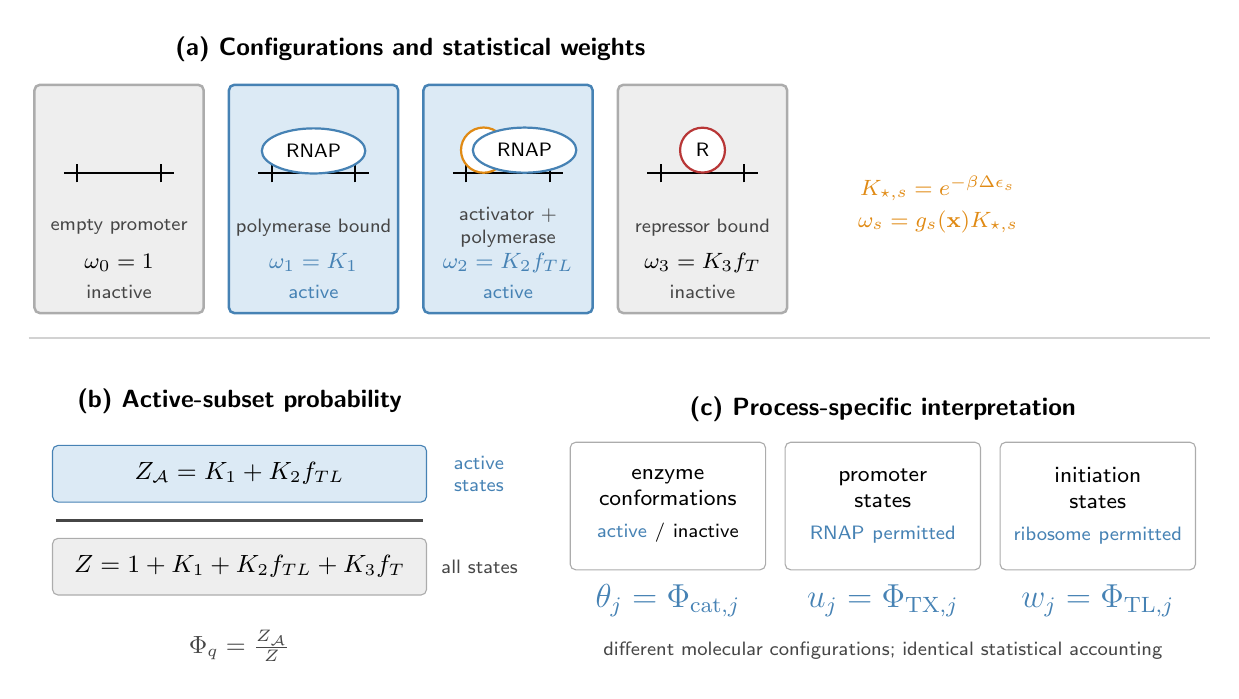
\begin{tikzpicture}[
  font=\small,
  paneltitle/.style={font=\bfseries\small, align=center},
  state/.style={rounded corners=2pt, minimum width=2.15cm,
                minimum height=2.90cm, inner sep=4pt, align=center,
                line width=0.9pt},
  active/.style={state, draw=activeblue, fill=activefill},
  inactive/.style={state, draw=gray!65, fill=inactivefill},
  note/.style={font=\scriptsize, align=center, text=inkgray},
  process/.style={rounded corners=2pt, draw=gray!65, fill=white,
                  minimum width=2.48cm, minimum height=1.62cm,
                  text width=2.20cm, align=center, inner sep=4pt,
                  font=\footnotesize},
]

% -------------------------------------------------------------------------
% Panel A: representative molecular configurations and their weights.
% -------------------------------------------------------------------------
\begin{scope}[shift={(0,0)}]
  \node[paneltitle] at (4.85,7.62) {(a) Configurations and statistical weights};

  \node[inactive] (empty) at (1.15,5.72) {};
  \draw[line width=0.8pt] (0.45,6.05) -- (1.85,6.05);
  \draw[line width=0.8pt] (0.62,5.93) -- (0.62,6.17);
  \draw[line width=0.8pt] (1.68,5.93) -- (1.68,6.17);
  \node[note] at (1.15,5.36) {empty promoter};
  \node[font=\footnotesize] at (1.15,4.91) {$\omega_0=1$};
  \node[font=\scriptsize, text=inkgray] at (1.15,4.54) {inactive};

  \node[active] (rnap) at (3.62,5.72) {};
  \draw[line width=0.8pt] (2.92,6.05) -- (4.32,6.05);
  \draw[line width=0.8pt] (3.09,5.93) -- (3.09,6.17);
  \draw[line width=0.8pt] (4.15,5.93) -- (4.15,6.17);
  \node[ellipse, draw=activeblue, fill=white, line width=0.8pt,
        minimum width=9mm, minimum height=5.5mm, font=\scriptsize]
        at (3.62,6.33) {RNAP};
  \node[note] at (3.62,5.36) {polymerase bound};
  \node[font=\footnotesize, text=activeblue] at (3.62,4.91)
        {$\omega_1=K_1$};
  \node[font=\scriptsize, text=activeblue] at (3.62,4.54) {active};

  \node[active] (activator) at (6.09,5.72) {};
  \draw[line width=0.8pt] (5.39,6.05) -- (6.79,6.05);
  \draw[line width=0.8pt] (5.56,5.93) -- (5.56,6.17);
  \draw[line width=0.8pt] (6.62,5.93) -- (6.62,6.17);
  \node[circle, draw=energyorange, fill=white, line width=0.8pt,
        minimum size=5.5mm, font=\scriptsize] at (5.78,6.34) {A};
  \node[ellipse, draw=activeblue, fill=white, line width=0.8pt,
        minimum width=9mm, minimum height=5.5mm, font=\scriptsize]
        at (6.30,6.34) {RNAP};
  \node[note] at (6.09,5.36) {activator +\\polymerase};
  \node[font=\footnotesize, text=activeblue] at (6.09,4.91)
        {$\omega_2=K_2f_{TL}$};
  \node[font=\scriptsize, text=activeblue] at (6.09,4.54) {active};

  \node[inactive] (repressor) at (8.56,5.72) {};
  \draw[line width=0.8pt] (7.86,6.05) -- (9.26,6.05);
  \draw[line width=0.8pt] (8.03,5.93) -- (8.03,6.17);
  \draw[line width=0.8pt] (9.09,5.93) -- (9.09,6.17);
  \node[circle, draw=repressred, fill=white, line width=0.8pt,
        minimum size=5.5mm, font=\scriptsize] at (8.56,6.34) {R};
  \node[note] at (8.56,5.36) {repressor bound};
  \node[font=\footnotesize] at (8.56,4.91) {$\omega_3=K_3f_T$};
  \node[font=\scriptsize, text=inkgray] at (8.56,4.54) {inactive};

  \node[font=\footnotesize, text=energyorange, align=center]
    at (11.55,5.65)
    {$K_{\star,s}=e^{-\beta\Delta\epsilon_s}$\\[2pt]
     $\omega_s=g_s(\mathbf x)K_{\star,s}$};
\end{scope}

\draw[gray!35, line width=0.6pt] (0,3.95) -- (15.00,3.95);

% -------------------------------------------------------------------------
% Panel B: active subset over all configurations.
% -------------------------------------------------------------------------
\begin{scope}[shift={(0,0)}]
  \node[paneltitle] at (2.68,3.15) {(b) Active-subset probability};

  \node[rounded corners=2pt, draw=activeblue, fill=activefill,
        minimum width=4.75cm, minimum height=0.72cm, align=center]
    (num) at (2.68,2.23)
    {$Z_{\mathcal A}=K_1+K_2f_{TL}$};
  \node[font=\scriptsize, text=activeblue, align=center, text width=0.9cm]
    at (5.72,2.23) {active\\states};

  \draw[line width=1.0pt, inkgray] (0.35,1.64) -- (5.01,1.64);

  \node[rounded corners=2pt, draw=gray!65, fill=inactivefill,
        minimum width=4.75cm, minimum height=0.72cm, align=center]
    (den) at (2.68,1.05)
    {$Z=1+K_1+K_2f_{TL}+K_3f_T$};
  \node[font=\scriptsize, text=inkgray, anchor=west]
    at (5.12,1.05) {all states};

  \node[font=\small, text=inkgray] at (2.68,0.04)
    {$\Phi_q=\frac{Z_{\mathcal A}}{Z}$};
\end{scope}

% -------------------------------------------------------------------------
% Panel C: the same accounting controls three biological processes.
% -------------------------------------------------------------------------
\begin{scope}[shift={(6.80,0)}]
  \node[paneltitle] at (4.05,3.05) {(c) Process-specific interpretation};

  \node[process] (cat) at (1.32,1.82)
    {enzyme\\conformations\\[2pt]
     {\scriptsize\textcolor{activeblue}{active} / inactive}};
  \node[font=\large, text=activeblue] at (1.32,0.62)
    {$\theta_j=\Phi_{\mathrm{cat},j}$};

  \node[process] (tx) at (4.05,1.82)
    {promoter\\states\\[2pt]
     {\scriptsize\textcolor{activeblue}{RNAP permitted}}};
  \node[font=\large, text=activeblue] at (4.05,0.62)
    {$u_j=\Phi_{\mathrm{TX},j}$};

  \node[process] (tl) at (6.78,1.82)
    {initiation\\states\\[2pt]
     {\scriptsize\textcolor{activeblue}{ribosome permitted}}};
  \node[font=\large, text=activeblue] at (6.78,0.62)
    {$w_j=\Phi_{\mathrm{TL},j}$};

  \node[note] at (4.05,-0.02)
    {different molecular configurations; identical statistical accounting};
\end{scope}

\end{tikzpicture}
\end{document}
